% This must be in the first 5 lines to tell arXiv to use pdfLaTeX, which is strongly recommended.
\pdfoutput=1
% In particular, the hyperref package requires pdfLaTeX in order to break URLs across lines.

\documentclass[11pt]{article}

% Remove the "guidelines" option to generate the final version.
\usepackage[guidelines]{nlpreport} % show guidelines
%\usepackage[]{nlpreport} % hide guidelines


% Standard package includes
\usepackage{times}
\usepackage{latexsym}



% For proper rendering and hyphenation of words containing Latin characters (including in bib files)
\usepackage[T1]{fontenc}
% For Vietnamese characters
% \usepackage[T5]{fontenc}
% See https://www.latex-project.org/help/documentation/encguide.pdf for other character sets

% This assumes your files are encoded as UTF8
\usepackage[utf8]{inputenc}

% This is not strictly necessary, and may be commented out,
% but it will improve the layout of the manuscript,
% and will typically save some space.
\usepackage{microtype}
\usepackage{graphicx}
\usepackage{hyperref}
\usepackage{amsmath}
\usepackage{mathtools}
\usepackage{multirow}
\usepackage{listings}
\usepackage{xcolor}
\usepackage{booktabs} % for tables
\usepackage{multicol}
\usepackage{adjustbox}
\usepackage{float}
\usepackage{caption}







% THE pdfinfo Title AND Author ARE NOT NECESSARY, THEY ARE METADATA FOR THE FINAL PDF FILE
\hypersetup{pdfinfo={
Title={Assignment 1},
Author={Federico Rullo}
}}
%\setcounter{secnumdepth}{0}  
 \begin{document}
%
\title{Assignment 1\\
% subtitle
}
\author{Fabio Zanotti,
Antonio Morelli,
Federico Rullo,
\and
Edoardo Conca\\
Master's Degree in Artificial Intelligence, University of Bologna\\
\{ fabio.zanotti, antonio.morelli, federico.rullo, edoardo.conca \}@studio.unibo.it
}
\maketitle

\begin{abstract}
%\begin{quote}

In this project, we present the implementation and evaluation of a Part-Of-Speech (POS) tagging system using neural architectures. We explore three different neural models: a baseline model with a single Bidirectional Long Short-Term Memory (LSTM) layer, an extended model with an additional Bidirectional LSTM layer, and a variant with an extra Dense layer.  The results showed how the deeper models behaved better than the baseline, although the simpler architecture performs comparably to the more complex models, which may suggest that the complexity introduced by the extra layers did
not provide substantial benefits for the task.

%\end{quote}
\end{abstract}

\section{Introduction}
\label{sec:introduction}
The assignment aims to develop a POS tagging system using neural architectures to predict the POS tag for each word in a corpus. Three models are implemented and compared to determine performance superiority. Bidirectional LSTM layers are utilized for contextual understanding, crucial for accurate POS tagging. Methodology involves model implementation and comparison using the average Macro-F1 score as a performance metric. Preprocessing includes dataset encoding and integration of GloVe embeddings for weight initialization, leveraging pre-trained representations. Out-Of-Vocabulary (OOV) words are incorporated into the vocabulary, with embeddings computed based on tag-specific means. Experimental evaluation indicates improved accuracy in models with additional Bidirectional LSTM or Dense layers, emphasizing enhanced contextual and feature representation in POS tagging.


\section{System description}
\label{sec:system}
The three different models implemented are:
\begin{itemize}
    \item Baseline - consisting of a single Bidirectional LSTM layer;
    \item Baseline with an additional Bidirectional LSTM layer,  to further capture contextual dependencies;
    \item Baseline with an additional Dense layer, to enhance the feature representation;
\end{itemize}
We started by importing the dataset from the Natural Language Toolkit(NLTK) library, which we pre-processed and then encoded, and removing the "-NONE-" tag, so that the model will have fewer examples of unstructured data to learn, and can focus on the examples that are most relevant to the POS tagging,increasing the accuracy of the results.
\\After inspecting the dataset composition, which seemed to be affected by some inbalance in between classes, we built the vocabulary; for this, we used the 100-dimensional version of GloVe to balance computational efficiency and semantic richness. Subsequently, these embeddings initialized the model's weights, leveraging pre-trained word representations to enhance our task's performance.
\\To address Out-Of-Vocabulary (OOV) words, the GloVe vocabulary was expanded by integrating OOV words from the dataset. Instead of just assigning random vectors to OOV words, tag-specific means from existing words were computed, ensuring meaningful embeddings and improving model performance. This process was iteratively applied to the training, validation, and test sets to compute the vocabulary.
\\Encoded sentences were padded to the length of the second-longest sentence, excluding the longest one because it turned out to be an outlier, and the padding label was defined as "-PAD-", following treebank notation.
\\Finally, we implemented the three models for the POS Tagging system. Each of these models have the same input and output layers, comprising GloVe Embedding as the input layer and TimeDistributed as the output layer. The differentiating factor among these models lies in their hidden layers.
The initial model, designated as the Baseline model, consists solely of a single Bidirectional LSTM hidden layer \ref{fig:baseline}.The second model extends the Baseline model by incorporating an additional Bidirectional LSTM layer \ref{fig:lstm}. And lastly, the third and ultimate model integrates an additional Dense layer into the Baseline architecture \ref{fig:dense}.



\section{Experimental setup and results}
\label{sec:results}

\subsection{Parameter Tuning}
Prior to conducting experiments, hyperparameter tuning was performed for each model. We observed significant effects on scores due to variations in LSTM layer units and batch size. Balancing model complexity and overfitting, we set the LSTM units between 128 and 256. A batch size of 32 was chosen to enhance performance, reduce variance, and address class imbalance. Consistency across models was ensured by employing the same parameters.
Callbacks were utilized for effective training control.
\subsection{Metrics}
Custom metrics were defined to accommodate non-informative classes in POS tagging evaluation. Classes such as punctuation and symbols were ignored, with custom metrics including a masked F1 macro score for post-training evaluation.
\\To address dataset imbalance, a custom accuracy metric was devised. This metric assigns different weights to errors on specific classes and computes accuracy accordingly. By excluding certain classes and adjusting weights, the metric provides a balanced evaluation of model performance.
\subsection{Results}
The following tables provide a clear comparison of model performances on both validation and test sets, highlighting the effectiveness of the Additional Dense model in improving macro F1 scores.
\begin{table}[ht]
\caption{Avg F1 Scores on Validation Set}
\centering
\begin{tabular}{|l|l|}
\hline
  & Macro F1 Scores \\ \hline
Baseline Model                     & 0.7891                   \\ \hline
Additional LSTM                    & 0.7966                   \\ \hline
Additional Dense                  & \textbf{0.7992}                   \\ \hline
\end{tabular}
\label{Tab:Tcr_1}
\end{table}


\begin{table}[ht]
\footnotesize
\caption{Avg F1 Scores on Test Set}
\centering
\begin{tabular}{|l|l|}
\hline
                             & Macro F1 Scores \\ \hline
Baseline Model                     & 0.7810                   \\ \hline
Additional LSTM                    & 0.7836                  \\ \hline
Additional Dense                  &  \textbf{0.7851}                   \\ \hline
\end{tabular}
\label{Tab:Tcr_2}
\end{table}


\section{Discussion}
\label{sec:discussion}
\subsection{Quantitative Results}
Upon analyzing the results, it is evident that while the performances of the two deeper models are comparable, the one with two Dense layers exhibits slightly superior performance on average. However, adhering to the outlined request for error analysis on the best single model based on the validation set performance, we focused on one of the LSTM models, which achieved a macro F1-score of 0.8054. This observation suggests that LSTM layers effectively captured sequential dependencies and long-range relationships within the input data, crucial for POS tagging tasks.

\subsection{Error analysis}
We observed a higher error rate on the validation set compared to the test set, possibly due to more challenging or edge case samples in the validation set. Four classes—NN, NNP, JJ, and NNS—were consistently among the top mismatches for each model, with their higher presence in the validation set explaining the increased error rate.
Investigating further, we found that errors predominantly occurred between classes with semantic and syntactic similarities, such as NN (Noun, singular or mass), NNP (Proper noun, singular), JJ (Adjective), and NNS (Noun, plural). Confusion between these classes stems from their overlapping characteristics, such as singular vs. plural forms and common vs. proper nouns.

\section{Conclusion}
\label{sec:conclusion}
Surprisingly, we found that the simpler Baseline
model performances are worse by a marginal factor of approximately $\approx 1\%$. This suggests that the
additional layers in the deeper models did not significantly improve performance. One possible explanation for this is that the complexity introduced
by the extra layers did not provide substantial benefits for the POS tagging task. It’s possible that the
Baseline model’s simpler architecture was already
effective in capturing the necessary patterns in the
data, leading to comparable performance despite
its simplicity



\section{Links to external resources}
\label{sec:links}
\href{https://github.com/antoniototimorelli/nlp_unibo_2023-24_assignments/tree/main/Assignment_1}{Assignment\_1}

\onecolumn
\section*{Appendix}
\subsection*{Figures}
\begin{figure}[H]
        \centering
        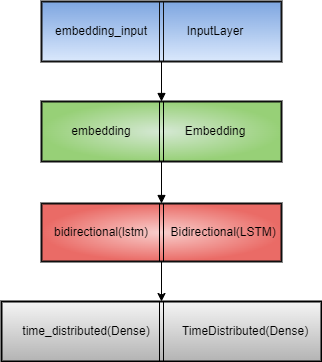
\includegraphics[scale=0.41]{img/Baseline.png}
        \caption{Baseline architecture}
        \label{fig:baseline}
\end{figure}

\begin{figure}[H]
        \centering
        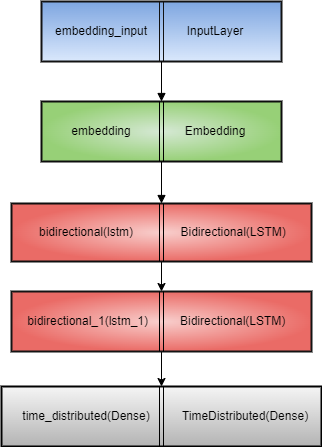
\includegraphics[scale=0.41]{report/img/Additional_lstm.png}
        \caption{Additional LSTM architecture}
        \label{fig:lstm}
\end{figure}

\begin{figure}[H]
        \centering
        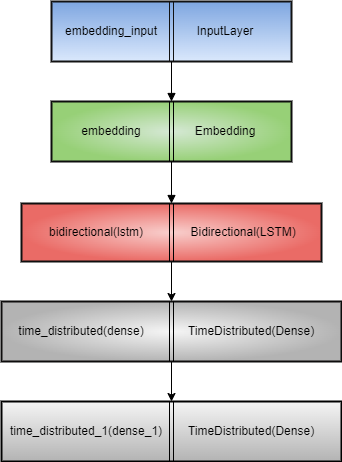
\includegraphics[scale=0.41]{img/Additional_dense.png}
        \caption{Additional Dense architecture}
        %\captionsetup{justification=centering, singlelinecheck=false}
        \label{fig:dense}
\end{figure}

\end{document}
\begin{multicols}{2}
\begin{minipage}[t]{0.40\textwidth}
\nocite{*}
\bibliography{nlpreport.bib}..
\end{minipage}

\begin{minipage}[t]{0.6\textwidth}
    \begin{figure}[H]
        \raggedleft
        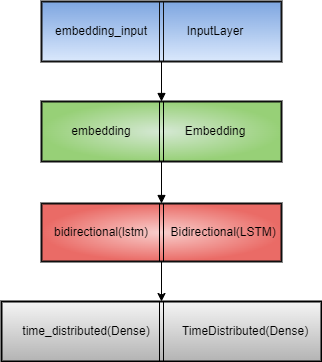
\includegraphics[scale=0.43]{img/Baseline.png}
        \caption{Baseline architecture}
        \label{fig:baseline}
    \end{figure}

    \begin{figure}[H]
        \raggedleft
        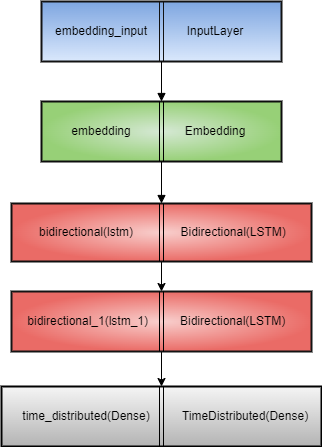
\includegraphics[scale=0.43]{report/img/Additional_lstm.png}
        \caption{Additional LSTM architecture}
        \label{fig:lstm}
    \end{figure}

    \begin{figure}[H]
        \raggedleft
        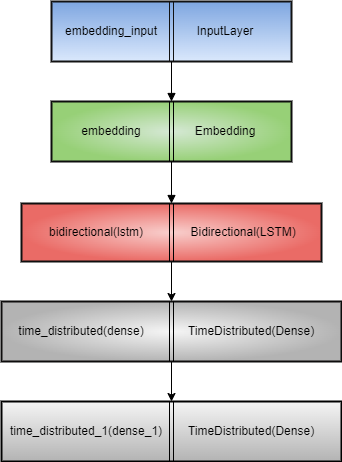
\includegraphics[scale=0.43]{img/Additional_dense.png}
        \caption{Additional Dense architecture}
        \label{fig:dense}
    \end{figure}
    \end{minipage}

\end{multicols}
